% !TeX root = ../main.tex
% %%%%%%%%%%%%%%%%%%%%%%%%%%%%%%%%%%%%%%%%%%%%%%%%%%%%%%%%%%%%%%%%%%%%%%%%%%%%%%
% Proposed Approach
\chapter{Proposed Approach}
\label{chap:approach}


The proposed approach consists initially in creating a specific language.
The language will serve as a way to describe the properties of a robot.
For instance, if our robot is an autonomous car navigating on the road, 
one property could be that the robot stops at stop signs.
To describe robot properties, we also need the description of the testing scenario.
In the above example, the "road" and "stop sign" should be defined in the language as part of the 
testing scenario, without it there would be no way to describe the above property effectively.

\par

Next in the approach, there is a need to build a compiler for the proposed language.
The compiler should be able to interpret a property in the language and be able to
identify the components of the robot necessary to monitor the said property.
The monitorization could take place either during runtime or after using log files.
Taking the above example into account, our compiler should have the information of which 
component of the robot is responsible for the car position as well as the position of the 
stop sign, it can then monitor the component and check if the property has been broken.

\par

The language should be of high level in the sense that it should be intuitive to the writer.
With this approach, the person doing the robot testing shouldn't need so much in-depth 
knowledge about the robot to perform a test. This is because of the writing simplicity of 
the language and the removal of the manual labor side of personally monitoring the robot.

*add GzScenic to the text somehow*

*TODO intro to the iamge and image*

%Maybe no image here
%\begin{figure}[h!]
%    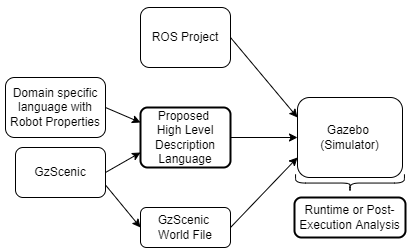
\includegraphics{images/intro_diag.png}
%    \caption{Tool for monitoring robot properties.}
%    \label{fig:intro_objectives}
%\end{figure}